\documentclass[12pt, letter]{report}

\usepackage{amsmath}    % need for subequations
\usepackage[pdftex]{graphicx}   % need for figures
\usepackage{verbatim}   % useful for program listings
\usepackage{color}      % use if color is used in text
\usepackage{caption}  
\usepackage{subcaption}  % use for side-by-side figures
\usepackage{hyperref}   % use for hypertext links, including those to external documents and URLs
\usepackage{setspace}
\doublespacing

\allowdisplaybreaks
\captionsetup{compatibility=false}

\graphicspath{{anatomy_figs/}}

\begin{document}
\section{Ethology of Rodent Ultrasonic Vocalizations}
To be a rodent is to be prey. A large number of vertebrate predators make use of rodents as a primary food source. Birds of prey are especially effective hunters, depleting local rodent populations in area before undertaking migrations to search for new hunting grounds. With these environmental pressure it is no wonder many rodents have evolved burrowing behaviors as a strategy for hiding from these dangers. However, specialized predators such as weasels have even evolved slender and elongated bodies to capture rodents from their burrows. Thus, even the relative safety of their nest areas can be ineffective protection. Some studies report that predation can have a staggering $95 \%$ impact on rodent populations \cite{Jedrzejewski1993}. With these considerations in mind, it is quite reasonable to expect that predation has been one of the driving factors in the evolution of rodent social behavior \cite{Brudzynski2010}. Perhaps one of the more powerful and complex evolutionary traits in vertebrates is that of vocal communication. As a results of their position in the food chain some rodent species have developed a peculiar form of vocal communication, one that lies entirely in the ultrasonic range. The advantage of this form of vocalization is the ability of an individual to communicate and provide warning to conspecifics with lowered risk of detection by predators. In this section I will discuss the origins of and behavior surrounding rodent ultrasonic vocalizations (USVs), more specifically those of rats. 

There is evidence that the phylogenetic origins of social vocalizations in vertebrates are over 400 million years old. Bass et al. have shown that the same vocal region in the caudal hindbrain and rostral spinal cord region is present in fish and all major lineages of vocal tetrapods \cite{Bass2008}. Rodent USV as a defensive adaptation is however a much more recent development. The suborder of myomorph rodent emerged about 40 million years ago, while the generas Mus and Rattus emerged as distinct groups between 16 and 23 million years ago. Species of both these generas use ultrasound for communication. Thus, it is likely rodent USV emerged somewhere between 20 and 40 million years ago. It is believed that the nocturnal lifestyle of the rodent predisposed them to evolve ultrasonic communication as a defensive strategy. Increased visual acuity is not beneficial to nocturnal animals. Thus, many rodents have evolved increased auditory acuity that extends into the ultrasonic range, and auditory sensitivity in the ultrasonic range is a prerequisite for communication in those frequencies.

It has been suggested by Blumberg and Alberts and then later by Hofer and Shair that rodent USVs originally evolved as a way for infants to help stimulate endogenous heat production. Blumberg and Alberts observed dur- ing vocalization closure of the larynx results in an increase in intrathoracic pressure, a phenomenon known as laryngeal braking. Under certain circum- stances laryngeal braking can increase pulmonary oxygenation of the blood. They hypothesized that this increased blood oxygen level could assist brown adipose tissue with increasing the body temperature of a hypothermic infant \cite{Blumberg1990}. In their 1992 paper, Hofer and Shair observed that when infant rats are brought into a comatose state of hypothermia, with a body of temperature of 20◦C, they will begin vocalizing in the ultrasonic range. When the comatose rat pup is placed in contact with their mother there is initially no change in the emission of USVs. However when their temperature warms to 25◦C they become responsive to the mother’s presence and cease vocalizing \cite{Hofer1992}. This suggests that infant USVs serve a dual purpose: to assist in raising the body temperature of a hypothermic pup and to summon the mother to a pup in distress. However, it does not conclusively determine the original evolutionary strategy surrounding infant USVs. To help elucidate this Hofer and Shair compared rising body temperature in two groups of hypothermic rat pups, a control group and a group devocalized through laryngeal denervation or tracheostomy. They found that the body temperature of the control group rose faster than the devocalized group, and $20 \%$ of the devocalized group did not recover at all. Autopsy of these specimens found pulmonary edema \cite{Hofer1993}. Thus it seems likely that USVs in rodents originally evolved as a strategy for increasing the body temperature in infant hypothermia and the maternal instinct to interpret that as a distress call arose later \cite{Hofer2010}.

In adult rodents ultrasonic vocalization requires complex laryngeal, prolonged exhalation, and increased lung pressure. These significant energy demands indicate the adaptive value of ultrasonic communication in avoiding detection by predators. The acoustic properties of vocalizations in the ultrasonic range confer this adaptive value. Because acoustic waves in the ultrasonic range spread at a lower rate than those in the sonic range, USVs allow individuals to better control the directionality of their calls. Ultrasonic acoustic waves also attenuate at a much higher rate in atmosphere and solid matter than sonic waves, minimizing the chance of detection by an outside predator. Furthermore, because rodents USVs are largely monotonal in frequency, it is more difficult to localize their source, another acoustic property that makes detection more difficult by a predator. These acoustic properties make USVs ideal for short-range communication with conspecifics inside of burrows \cite{Brudzynski2007a}.

Rat species are commonly used when studying rodent USVs. This is because of the ease of laboratory handling and their highly social nature. Adult rats exhibit a large repertoire of USVs. One of the most easily recognizable of their USVs is the 22 khz alarm call (Fig. \ref{fig:22_khz}). This type of vocalization is elicited by the presence of a predator or by social defeat. Blanchard et al. were able to observe these calls in burrowing lab rats when exposed to a cat \cite{Blanchard1991}. Panksepp et al. were also able to observe this type of call after Long-Evans rats submitted to more socially aggressive conspecifics in a laboratory setting \cite{Panksepp2007}. Brudzynski and Brihari were able to artificial stimulate $22-kHz$ alarm calls by intracerebral injection of acytelcholine agonist carbachol, which is known to cause an acute stress response \cite{Brudzynski1990}. \cite{Burgdorf2010}. 

Another distinct group of rat USVs lie in the $50-85$ kHz range. They are associated with positive social interactions with conspecifics (mating and playful fighting) and anticipation of food. Aversive stimuli such as social defeat, frustrating situations, and electrical shock decrease the number of calls emitted in this range. Mu-opiate and dopamine agonists as well as electrical stimulation of the mesolymbic dopamine system also elicit calls in this frequency region  \cite{Burgdorf2010}. The calls in this region exhibit considerable variability. Beyond signifying positive emotional states it is not entirely certain what information they are encoding. 
\begin{figure}
\centering
\includegraphics[width=0.5\linewidth]{22_khz.png}
\label{fig:22_khz}
\end{figure}
\begin{figure}
\centering
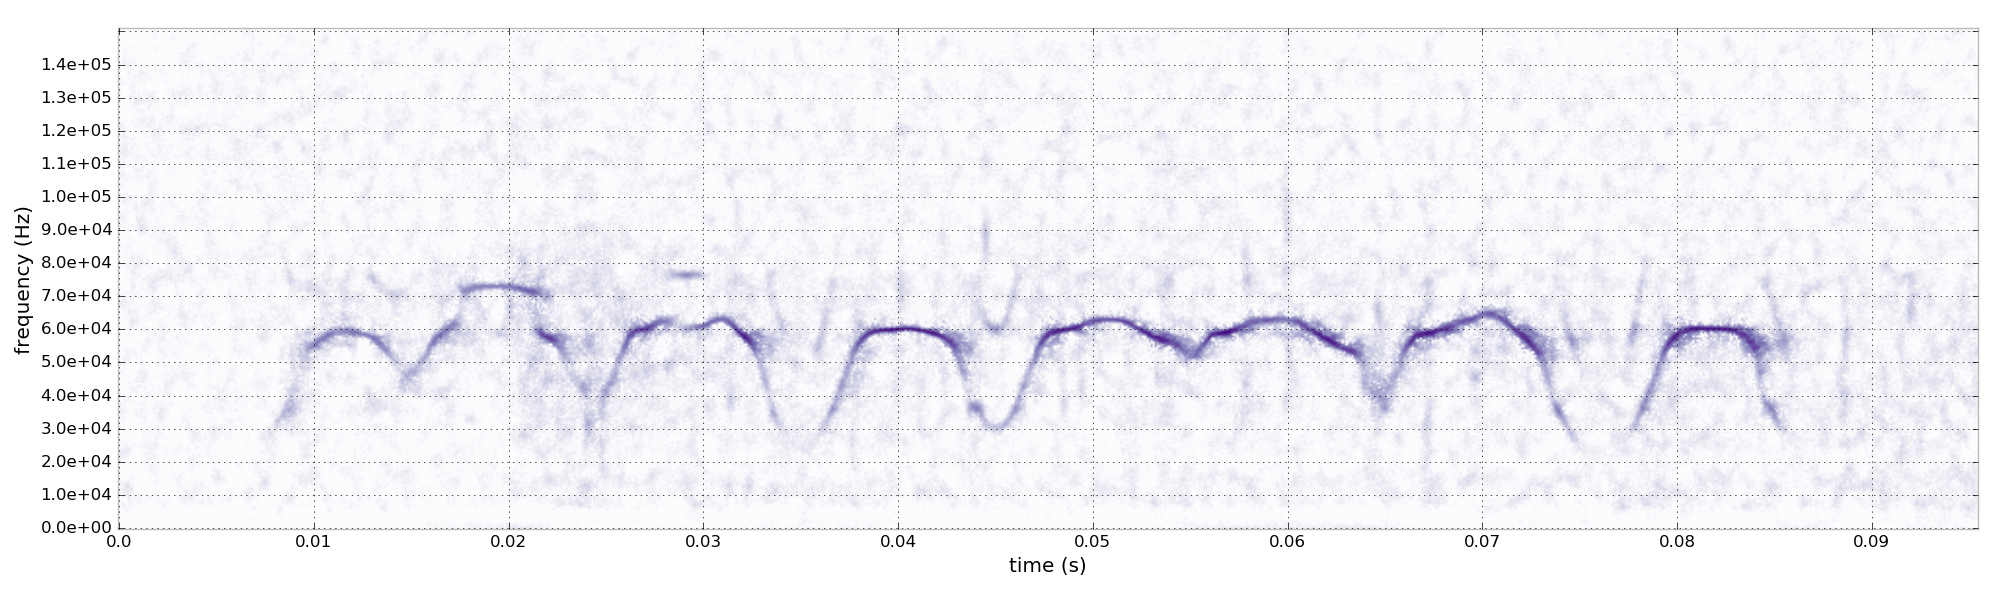
\includegraphics[width=\linewidth]{60_khz_trill.png}
\end{figure}
\begin{figure}
\centering
\includegraphics[width=\linewidth]{flat_to_trill.png}
\end{figure}
\begin{figure}
\centering
\includegraphics[width=\linewidth]{flat_to_trill_to_flat.png}
\end{figure}

\section{Anatomy of the Larynx}
The essential structure of the larynx is mostly conserved throughout mammals. It consists of a cartilagenous framework, extrinsic laryngeal muscles, which connect the framework to its surroundings in the body, and smaller intrinsic laryngeal muscles, which lie entirely inside the larynx. The cartilage framework consists of the cricoid, thyroid, and arytenoid cartilages (Fig. \ref{fig:laryngeal_cartilage}). The cricoid cartilage is ring like in shape and sits at the top of the trachea. The thyroid cartilage, also known as the Adam’s apple, attaches to the cricoid cartilage posteriorly. It posses a few degrees of articulation. At the top of cricoid cartilage ring sit the arytenoid cartilages. They are roughly pyramidal in shape and have complex rotational articulations. Two sets of intrinsic laryngeal muscles, the posterior and lateral cricoarytenoid muscles, attach the arytenoid cartilages to the cricoid cartilage: and are responsible for their abduction and adduction. Adduction of arytenoids occurs during swallowing, to prevent debris from entering the trachea, and during phonation, to set the vocal folds in a position in which they can oscillate. Adduction occurs when the lateral cricoarytenoid muscles, attached to the front of the cricoid, con- tract, causing the arytenoids to rotate inward. The interarytenoid muscles, which as its name suggest lies in between the arytenoids assists with this process. Abduction occurs during inspiration and occurs when the posterior cricoarytenoid muscles contract rotating the arytenoids outward \cite{Berke2010}. The thyroarytenoid muscles attach at the arytenoids anteriorly and run to the thyroid cartilage posteriorly. These muscles are covered with a layer of connective tissue. Collectively this muscles and connective tissue structure are called the vocal folds. In common speech this structure is called the vocal cords, which is somewhat of a misnomer, since they are not chord shape, nor do they generate sound in the manner of a vibrating guitar string. As mentioned above, rotation of the arytenoids can abduct and adduct the vocal folds by contraction of the cricoarytenoid and interarytenoid muscle. Contraction of the thyroarytenoid muscles themselves can further adduct the vocal folds, in addition to shortening them by rotating the arytenoids inward. Contraction of the cricothyroid muscles can lengthen the vocal folds. A total of five muscles contribute to the movement of and tension of the vocal folds. Considering the small size of the structure this is a remarkable degree of control, which is used for the complicated process of vocalization. Fig. 2 shows an illustration of the intrinsic laryngeal muscles \cite{Berke2010}. 
\begin{figure}
\centering
\begin{subfigure}[b]{0.4\linewidth}
\centering
\includegraphics[width=\linewidth]{larynx_ligaments_antero_lateral.png}
\caption{}
\end{subfigure}
\begin{subfigure}[b]{0.4\linewidth}
\centering
\includegraphics[width=\linewidth]{larynx_ligaments_posterior_view.png}
\caption{}
\end{subfigure}
\caption{Ligaments of the larynx (a) antero-lateral view (b) posterior view \cite{Gray2000Anatomy}}
\label{fig:laryngeal_cartilage}
\end{figure}

\begin{figure}
\centering
\begin{subfigure}[b]{0.4\linewidth}
\centering
\includegraphics[width=\linewidth]{larynx_muscles_top.png}
\caption{}
\end{subfigure}
\begin{subfigure}[b]{0.4\linewidth}
\centering
\includegraphics[width=\linewidth]{larynx_muscles_side.png}
\caption{}
\end{subfigure}
\caption{(a) Top view of the laryngeal muscles (b) Side view of the laryngeal
muscles. Shown in both (a) and (b) are the thyroarytenoid muscles, the
interarytenoid muscles (arytanoideus), the posterior cricoarytenoid muscles,
and lateral cricoarytenoid muscles. Shown only in (b) is the cricothyroid
muscle \cite{Gray2000Anatomy}.}
\label{fig:laryngeal_muscles}
\end{figure}

Innervation of the vocal fold musculature is completely supplied by the vagus nerve. Efferent motor fibers of the nerve emerge from the nucleus am- biguus in the medulla oblongata. Afferent sensory fibers of the nerve also terminate there. At the root of the neck the vagus branches into left and right components (?). Each component branches again into the superior laryngeal nerve (SLN) and the recurrent laryngeal nerve (RLN). The RLN contains only motor fibers, while the SLN contains both motor and sensory fibers. The SLN runs to the larynx, where it divides into the external and internal branches. The external branch provides motor control to the cricothyroid muscle. The internal branch carries sensory information from the mucosa lining, larynx, epiglottis, and part of the tongue. It enters the larynx through the thyrohyoid membrane. The left and right RLNs branch from the vagus nerve low in the neck. Upon reaching the larynx the RLNs branch again, innervating the posterior cricothyroid muscles, lateral cricothyroid muscles, interarytenoid muscle, and the thyroarytenoid muscle \cite{Damrose2003}. Fig. \ref{fig:vagus_nerve} illustrates the path taking by the branchings of the vagus nerve. The order of branching is stereotyped, but the precise branching pattern can vary between individuals. Each laryngeal muscle can be individually controlled by the human motor cortex. Such a high degree of control is indicative of the large evolutionary advantage imparted by vocal communication \cite{Berke2010}. 

\section{Physics of Vibrating Vocal Folds}
Phonation is the physical process underlying vocalization. It is the process by which the vocal folds produce sound through vibration. The basics physics and physiology underlying phonation are as follows. Stimulation of the intrinsic laryngeal muscles from the RLN causes the vocal folds to adduct into a closed position with a converging profile. With the vocal folds in a closed position, air flow from the lungs results in an increase in subglottal pressure. Because the of the converging profile, this increase in subglottal pressure will force the vocal folds apart. The inferior portion of the vocal folds open first. A wave, compressing the tissue laterally, travels upward to the superior portion of the vocal fold. This is called a mucosal wave. The forcing apart of the vocal folds causes an increase in airflow, which corresponds to a drop in the pressure holding them open. Abduction will continue until this pressure can longer balance the elastic restoring force of the vocal fold tissue. At this point the vocal folds will begin to close. Their most inferior points will collide before returning to their closed position with a converging profile, when the cycle will start again \cite{Titze2000, Berke2010}.
\begin{figure}
\centering
\includegraphics[width=0.5\linewidth]{vagus_nerve.png}
\caption{The vagues nerve \cite{Gray2000Anatomy}}
\label{fig:vagus_nerve}
\end{figure}

Detailed studies have been preformed indicating the sound properties of vocalizations can be controlled through activity of the laryngeal muscles. In most models the cricothyroid and thyroarytenoid are the most import muscles for control of vocal acoustics. Studies have shown activation of the cricothyroid muscle increases the fundamental frequency $f_0$ of vibration by increasing the internal tension of the vocal folds. The role of the thyroary- tenoid muscle in the modulation of $f_0$ is less clear. Studies in canines show $f_0$ increases with thyroarytenoid activation when $f_0$ is in the modal register but decreases when $f_0$ is the falsetto register \cite{Berke2010, Titze2000, Choi1993}. The body-cover theory proposed by Hirano and advanced by Titze attempts to explain modulations of fundamental frequency as a function of cricothyroid and thyroarytenoid muscle activation. The body-cover theory states that two distinct layers of tissue contribute to vocal fold tension differently. The outer layer, the cover, is composed of epithelial tissue as well as the superficial and intermediate layers of the lamina propria. The cover has not contractile properties, and thus it’s tension is completely controlled by the vocal fold length. The inner group, the body, is composed of the deep layers of the lamina propria and the thyroarytenoid muscle. It’s tension is not only determined by length but also by the active contractile properties of the thyroarytenoid muscle. Thus activation of the thyroarytenoid muscle can shorten the vocal folds but still cause an increase in $f_0$ due to an increase in internal stiffness of the muscle fibers \cite{Titze1988}.

A simple rod model of the thyroid and cricoid cartilages with forces acting on them due to laryngeal muscle activation leads to the following expression for fundamental frequency $f_0$
\begin{equation}
\begin{split}
f_0 &= f_{0p}\left( 1 + \frac{A_a}{A}\frac{\sigma_{am}}{\sigma_p} a_{ta} \right)^\frac{1}{2} \\
\sigma_p &= 4 L_0^2 \left( 1 + \epsilon \right)^2 f_{0p}^2 \\
f_{0p} &= 38 + 175 (\epsilon + 1) + 2450 (\epsilon + 1)^2 + 2 p_s \\
\epsilon &= 0.2 (1.5 a_{ct} - a_{ta}) 
\end{split}
\end{equation}
Here $a_{ta}$ and $a_{ct}$ are the activation percentages of the thyroarytenoid and cricothyroid muscles, $f_{0p}$ is the fundamental frequency for passive tissue (i.e for $a_{ta}=0$), $\sigma_p$ is the mean passive stress over the entire vibrating cross section A, $\sigma_{am}$ is the maximum active stress in the muscular cross section $A_a$ , $L_0$ is the passive length of the vocal folds, $\epsilon$ is the vocal fold strain, $\rho$ is the vocal fold density, and $p_s$ is the subglottal pressure. The numerical constants were obtained through experimental data fitting. A plot of $f_0$ as a function of thyroarytenoid and cricothyroid muscle activation can be seen in Fig. \ref{fig:f0_vs_ata} From the figure it can be seen that complex modulations of fundamental frequency can be obtained through activation of these muscles. Additionally it can be seen that while activation of the cricothyroid muscle usually corresponds to an increase in $f_0$ , activation of the thyroarytenoid muscle can lead to more complicated behavior \cite{Titze1988}.
\begin{figure}
\centering
\includegraphics[width=\linewidth]{f0_vs_ata.png}
\caption{Fundamental frequency $f_0$ plotted against thyroarytenoid muscle activation $a_{ta}$ for different values of cricothyroid muscle activation act ( $\frac{A}{A_a}=0.5$ $sigma_p= 100$ kPa , $p_s = 8 $ cm H20, $L_0 = 1.5$ cm ). From this figure it can be seen complex modulations of $f_0$ can be performed through activation of these muscles. }
\label{fig:f0_vs_ata}
\end{figure}

While the body-cover theory can explain variations of fundamental frequency as a result of vocal fold tension and subglottal pressure it is not sufficient to account for the harmonic content of vocalizations and their transient time behavior. To account for these complexities time domain oscillator models of the vocal folds must be considered. Fig. \ref{fig:vocal_folds_spring} shows a single mass model for the vocal folds. In his 1998 paper, Titze derived an equation that describes the small amplitude oscillations of a single mass model of the vocal folds.
\begin{equation} 
\begin{split}
m \ddot{x} + b \dot{x} + k x &= p_g \\
p_g &= p_s + (p_s - p_i) \left( 1 - \frac{a_2}{a_1} - k_e \right) / k_t \\
a_1 &= 2 L (x_{01} + x + \frac{\delta}{2c} \dot{x}) \\
a_2 &= 2 L (x_{02} + x - \frac{\delta}{2c} \dot{x})
\end{split}
\end{equation}
where $x$ is the displacement of the vocal folds from their equilibrium position, $m$ is their mass per unit area, $b$ is the coefficient of linear dissipation per unit area, $k$ is the restoration constant per unit area, $p_g$ is the intraglottal pressure, $p_s$ is the subglottal pressure, $p_i$ is the superglottal pressure, $a_1$ is the inferior area of the vocal folds, $a_2$ is the superior area of the vocal folds, $k_e$ is the pressure recover coefficient for the turbulent expansion region above the vocal folds, $k_t$ is the transglottal pressure coefficient, $L$ is the axial length of the vocal folds, $T$ is their traverse thickness, lastly $x_{01}$ and $x_{02}$ are the equilibrium displacements of the inferior and superior portions of the vocal folds respectively. Since the harmonic content of an acoustic wave in the vocal tract is determined by the oscillations of the vocal folds, the time course of a vocalization can be described using this model as a function of physiological parameters. The strength of the forcing is determined by the subglottal pressure $p_s$ and the glottal areas $a_1$ and $a_2$. The fundamental frequency $f_0 = \frac{1}{2 \pi} \sqrt{\frac{k}{m}}$ can be calculated using the body cover model and is thus determined by vocal fold tension and subglottal pressure. In addition, the effects of the upper vocal tract can be taken into account by the pressure $p_i$.    

\begin{figure}
\centering
\includegraphics[width=0.5\linewidth]{vocal_folds_spring.png}
\caption{Single mass model of the vocal folds (awaiting permission to reprint)}
\label{fig:vocal_folds_spring}
\end{figure}

While Titze's equations are successful in accounting for the transfer of kinetic energy of air into vocal fold oscillations, they are only valid for small displacements from the vocal folds' equilibrium positions. Several attempts have been made to introduce nonlinearities into these oscillator equations. The nonlinearities model the loss of energy due to collision of the vocal folds upon large deviations from their equilibrium positions. They have the affect of keeping solutions bounded and introducing harmonic content not accounted for by the fundamental frequency. One of the simpler, yet feature rich, attempts has been proposed by Magnasco et al to model oscillations of vocal folds in bird syrnixes. The Magnasco model basically consists of the Titze model with the introduction of a nonlinearity cubic in the vocal fold velocity.
\begin{equation} 
\label{eq:magnasco_model}
m \ddot{x} + b \dot{x} + \beta \dot{x}^3 + k x = p_s \frac{a_0 - b_0 + 2 \tau \dot{x}}{x + b_0 + 2 \tau \dot{x}},
\end{equation}
where here $\tau$ is treated as phenomenological constant. The Magnasco model predicts that the onset of vocal fold oscillations occur through a Hopf bifurcation, which can be achieved by varying the subglottal pressure $p_s$ and vocal fold stiffness $k$ (Fig. \ref{fig:magnasco_hopf}) \cite{Gardner2001}. Furthermore, the model was able to qualitatively reproduce the features of actual canary songs through simple modulations of these parameters  \cite{Gardner2001}.
\begin{figure}
\centering
\includegraphics[width=0.5\linewidth]{magnasco_hopf.png}
\caption{Bifurcation diagram for Eq. \ref{eq:magnasco_model}. The system is brought in an out of a state of self-oscillation through a Hopf bifurcation by varying the parameters $k$ and $p_s$ (reprinted with permission) \cite{Gardner2001}.}
\label{fig:magnasco_hopf}
\end{figure}
\begin{figure}
\centering
\includegraphics[width=0.5\linewidth]{magnasco_bird_song.png}
\caption{Qualitative features of canary song reproduced through simple variations of the parameters $k$ and $p_s$ (reprinted with permission) \cite{Gardner2001}.}
\label{fig:magnasco_hopf}
\end{figure}
\section{The Failure of Vibrating Vocal Fold Models for Ultrasonic Vocalizations}
The frequency of sonic mammalian vocalizations scales with species mass, according to a power law, over several orders of magnitude of size. This can be seen in Fig. \ref{fig:scaling_law}. The dashed line in the figure is a scaling law proposed by Bradbury and Vehrenkamp. They reasoned that call frequency should be proportional to the inverse of the linear scale of an animal, $f\propto L^{-1}$. Since $L$ is proportional the cube of the mass $M$ of the animal we get $f\propto M^{-3}$ \cite{bradbury1998principles}. It can be seen that while this scaling law does fit the general trend of the sonic data (purple boxes) agreement is not perfect.

A more accurate scaling law (the solid line) was derived by Fletcher by considering the optimal call frequency for an animal to make when it is a given distance away from a conspecific. If $A_v$ is the amplitude of oscillation of the vocal fold area, then from Bernoulli's law the amplitude of oscillation of the velocity of airflow through the vocal folds is given by
\begin{equation}  
U = \left( \frac{2p}{\rho} \right)^\frac{1}{2}A_v,
\end{equation}
where $p$ is lung pressure and $\rho$ is the density of air. We can think of the vocal folds as a circular aperture set in an infinite plane baffle. The effect of this is to ensure sound only radiates off into infinity in one direction and does not travel backwards. The acoustic power radiated as a function of frequency $f$ is then given by
\begin{equation}
\label{eq:power_generated}
P = \frac{\pi \rho f^2 U^2}{2 c},
\end{equation}
where c is the speed of sound in air. Sound amplitude decreases with distance according to an inverse square law. In addition, intensity decreases due to atmospheric absorption. Combining these effects the sound intensity as a function of distance from its source is given by
\begin{equation}
\label{eq:intensity_generated}
I(r) = \frac{P}{4 \pi r^2} e^{-\alpha f^1.5 r},
\end{equation}
where $\alpha=3.6 \times 10^{-8} m^{-1} Hz^{-1.5}$ is constant that takes into the account the effects of atmospheric absorption. The acoustic signal provided to the cochlea of a listening conspecific a distance $r$ from the vocalizer is given by
\begin{equation}
\label{eq:signal_received}
S(r) = I(r) A_E,
\end{equation}
where $A_E$ is the cross-sectional area of the outer ear. Combings Eqs. \ref{eq:power_generated}, \ref{eq:intensity_generated}, and \ref{eq:signal_received} we get,
\begin{equation}
\label{eq:signal_received2}
S(r) = \frac{p f^2 A_V^2 A_E}{4 c r^2} e^{-\alpha f^1.5 r}.
\end{equation}
It is required that $S(r) \geq T$f or the signal to be audible by a conspecific at a distance $r$ from the source, where $T$ is a threshold value that does not vary much between species. From Eq. \ref{eq:signal_received2} it can be seen the amplitude of the signal received at a distance $r$ varies as a function of frequency. To find the optimal frequency $f^*$ for communicating at range $r^*$ we require $\frac{\partial r}{\partial f}=0$ with $S(r^*)=T$. The optimization condition is satisfied when $\alpha f^n r = \frac{2}{n}$. Substituting this back into Eq. \ref{eq:signal_received2} and solving for $f^*$ we get,
\begin{equation}
f^*= \left( \frac{16 c T}{\alpha^2 n^2 A_V^2 A_E p} \right)^\frac{1}{2n+2}
\end{equation}
Assuming the mouth and ear diameters are proportional to the linear body dimension $L$ gives the result $f^* \propto L^{-\frac{3}{n+1}}$. Since the animals' mass is pr optional to $L^3$ this is equivalent to saying $f^* M^{-\frac{1}{n+1}}$. For the approximate value of $n=1.5$, this becomes $f^* \propto M^{-0.4}$ \cite{Fletcher2010}.
\begin{figure}
\centering
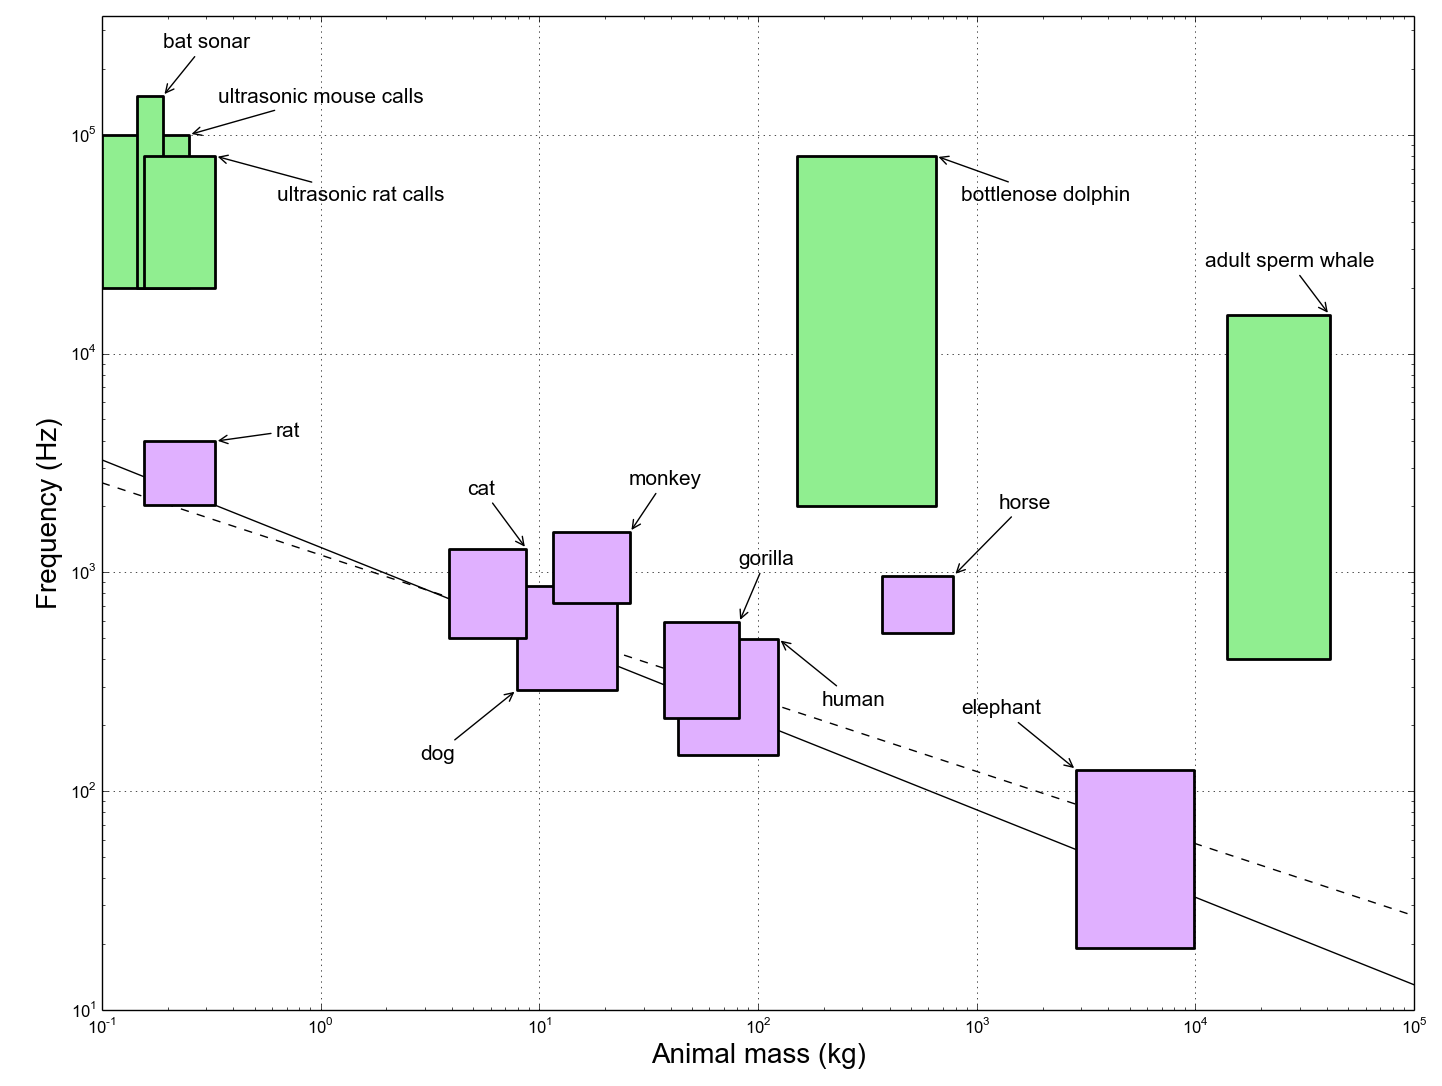
\includegraphics[width=0.5\linewidth]{frequnecy_scaling2.png}
\label{fig:frequency_scaling} 
\caption{Frequency scaling for mammals across several magnitudes of size (adapted from \cite{Fletcher2010}). The purple boxes show the ranges of audible frequencies emitted by several mammals plotted against the ranges of their masses. The solid and dotted lines show plots of a frequency scaling law of the form $f\propto M^{-\alpha}$. The dotted line ($\alpha=\frac{1}{3}$) is based on the conjecture that the average frequency emitted in audible vocalizations should be inversely proportional to the linear scale of the animal. The solid line ($\alpha=0.4$) is based on more in depth acoustic analysis to find the most efficient vocalization frequency for an animal of a given size. The green boxes show the range of ultrasonic frequencies emitted by several mammalian species plotted against their masses. These vocalizations do not obey the scaling laws \cite{white1998,berry1970natural,Fenton1998,Jones2006,bogdanowicz1994,Frankel2009,Whitehead2009,Rendell1999,Kastelein2000,Jefferson1993}.}
\label{fig:scaling_law}
\end{figure}
It can be seen the solid line fits the data for sonic vocalization very well across several orders of magnitude of size, indicating the same mechanisms for vocal production and audition are used throughout different species of mammals. However, it is also quite apparent that the data for ultrasonic vocalizations (green boxes) completely diverge from the scaling law. This is indicative of the fact the mechanisms for USVs are fundamentally different from that for sonic vocalizations.

In 1975 Roberts presented the first evidence that indicated vibrating vocal fold models were insufficient to describe USVs. In the study he placed young rats in a polyethylene bag and recorded both their sonic and ultrasonic vocalizations when the bag was filled with air. He then replaced the air with a heliox gas mixture of $20\%$ oxygen and $80\%$ helium. The effect of this is to increase the speed of sound in the bag by a factor of $1.7$. For the sonic vocalizations, when the bag, he observed that although the higher harmonics increased in frequency the fundamental frequency remained constant. This is consistent with the vibrating fold model, since the harmonic content will be determined by resonance properties of the vocal tract, but the fundamental frequency will be determined by the oscillations of the vocal folds. However for ultrasonic vocalizations, he observed an increase in fundamental frequency when air was replaced with heliox gas \cite{Roberts1975}. In 2011 Riede performed a more sophisticated version of this experiment. He inserted a metal tube into the trachea of several rats. The tube was capable of measuring subglottal pressure and injecting gas into the trachea. He injected a heliox mixture into the trachea of rats mid 22-kHZ vocalization and found an increase in fundamental frequency. Furthermore, he found the fundamental frequency increased in proportion to the amount of heliox gas present \cite{Riede2011}. 
This is inconsistent with a vibrating vocal fold model and indicates the source of oscillation is aerodynamic rather than physical in nature .

\bibliographystyle{prsty}
\bibliography{mdornfe1.bib}

\end{document}